

\tikzset{every picture/.style={line width=0.75pt}} %set default line width to 0.75pt        

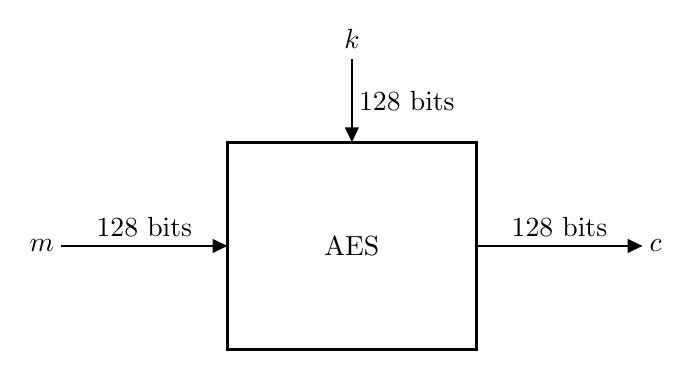
\begin{tikzpicture}[x=0.75pt,y=0.75pt,yscale=-1,xscale=1]
%uncomment if require: \path (0,300); %set diagram left start at 0, and has height of 300

%Shape: Rectangle [id:dp8114767489900245] 
\draw  [line width=1.2]  (100,60) -- (220,60) -- (220,160) -- (100,160) -- cycle ;
%Straight Lines [id:da8384818333827422] 
\draw    (20,110) -- (97,110) ;
\draw [shift={(100,110)}, rotate = 180] [fill={rgb, 255:red, 0; green, 0; blue, 0 }  ][line width=0.08]  [draw opacity=0] (7.14,-3.43) -- (0,0) -- (7.14,3.43) -- cycle    ;
%Straight Lines [id:da3063098296545941] 
\draw    (220,110) -- (297,110) ;
\draw [shift={(300,110)}, rotate = 180] [fill={rgb, 255:red, 0; green, 0; blue, 0 }  ][line width=0.08]  [draw opacity=0] (7.14,-3.43) -- (0,0) -- (7.14,3.43) -- cycle    ;
%Straight Lines [id:da9644541206291637] 
\draw    (160,20) -- (160,57) ;
\draw [shift={(160,60)}, rotate = 270] [fill={rgb, 255:red, 0; green, 0; blue, 0 }  ][line width=0.08]  [draw opacity=0] (7.14,-3.43) -- (0,0) -- (7.14,3.43) -- cycle    ;

% Text Node
\draw (160,110) node   [align=left] {AES};
% Text Node
\draw (60,107) node [anchor=south] [inner sep=0.75pt]   [align=left] {$\displaystyle 128$ bits};
% Text Node
\draw (260,107) node [anchor=south] [inner sep=0.75pt]   [align=left] {$\displaystyle 128$ bits};
% Text Node
\draw (162,40) node [anchor=west] [inner sep=0.75pt]   [align=left] {$\displaystyle 128$ bits};
% Text Node
\draw (18,110) node [anchor=east] [inner sep=0.75pt]    {$m$};
% Text Node
\draw (302,110) node [anchor=west] [inner sep=0.75pt]    {$c$};
% Text Node
\draw (160,16.6) node [anchor=south] [inner sep=0.75pt]    {$k$};


\end{tikzpicture}